The final step in the process is the controlled placement of the bent parts in storage or shelves. The robot system is integrated with a shelving control mechanism, which assigns each finished part a specific storage location based on its dimensions and characteristics.

Using a predefined pattern, the robot places each part onto the shelf, ensuring optimal space utilization. This process also keeps track of the number of parts produced and stored, with automatic alerts if the shelves reach capacity.

In the event that a shelf is full, the system can dynamically assign a new storage location or pause the production until the storage is made available again.

This final stage ensures that the entire workflow—from pickup, bending, inspection, to shelving—is seamlessly integrated and automated, maximizing efficiency and accuracy.

\begin{figure}[h]
    \centering
    \begin{subfigure}[b]{0.32\textwidth}
        \centering
        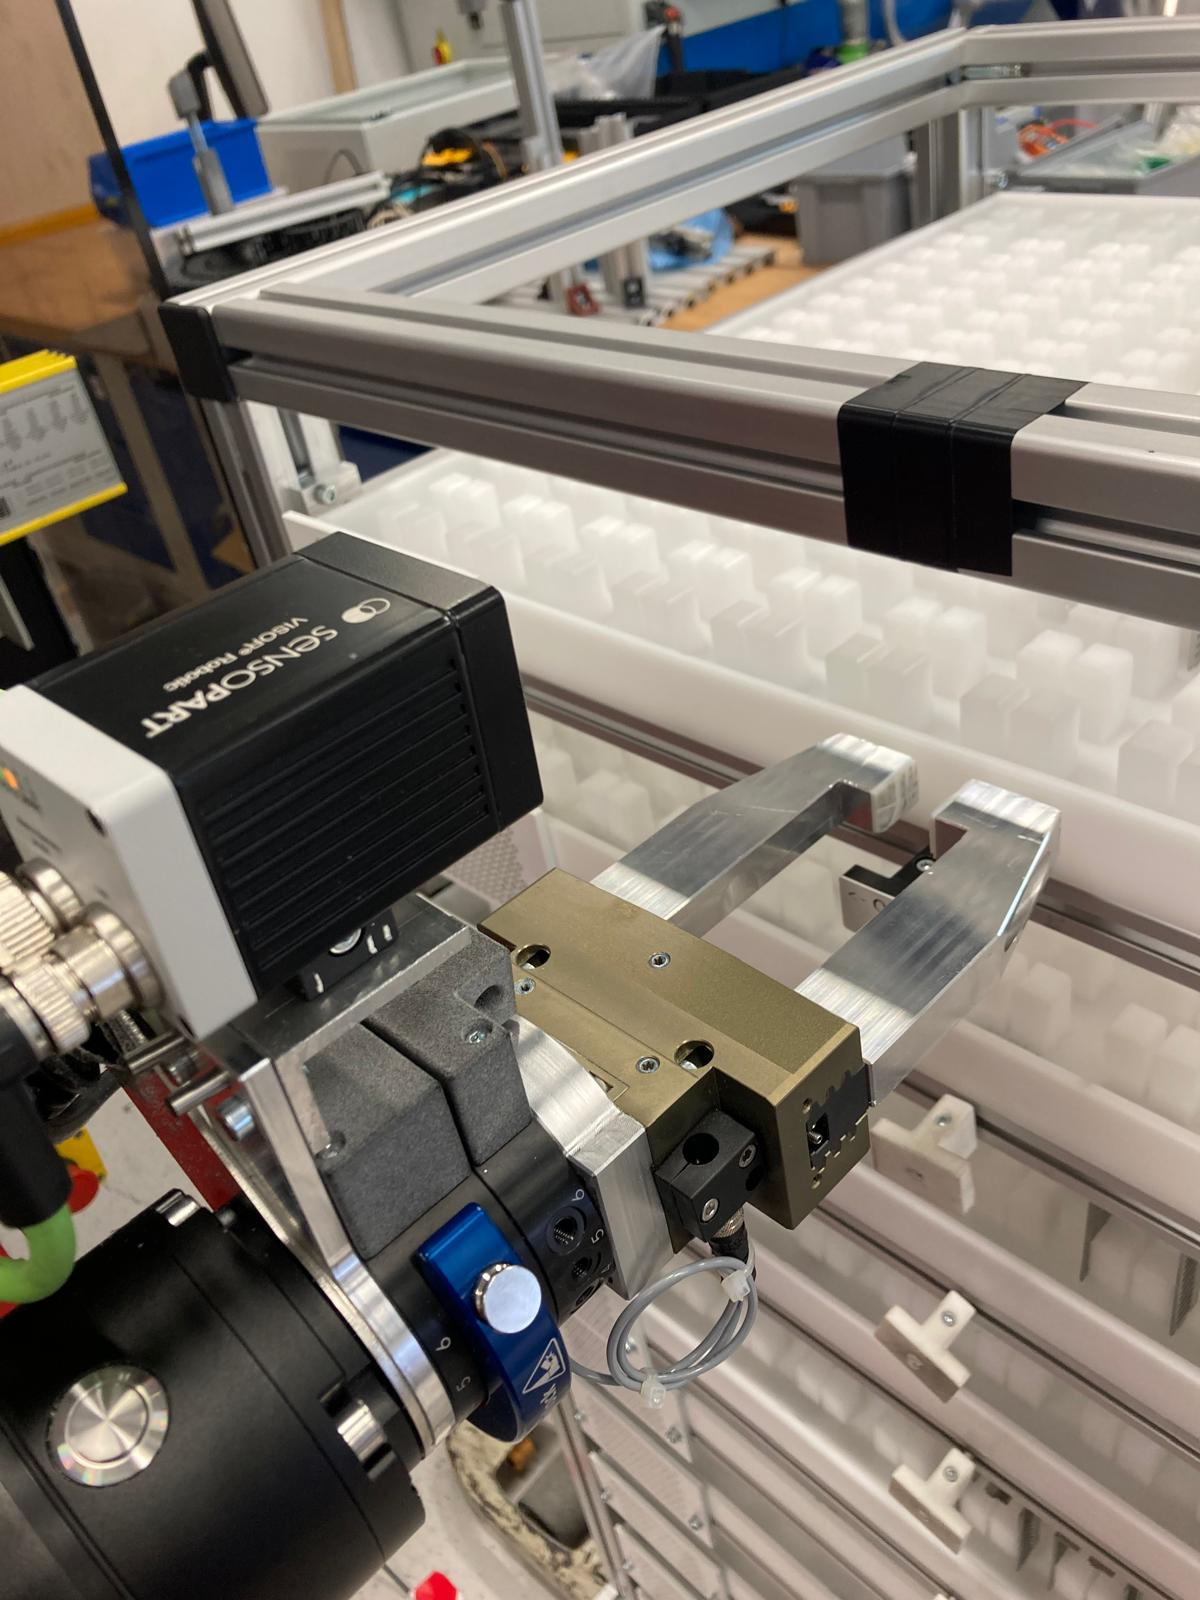
\includegraphics[width=\textwidth]{figures/shelf-control/reach-handle.jpeg}
        \caption{Reach shelf handle}
        \label{subfig:reach-handle}
    \end{subfigure}\hspace{0.1cm}
    \begin{subfigure}[b]{0.32\textwidth}
        \centering
        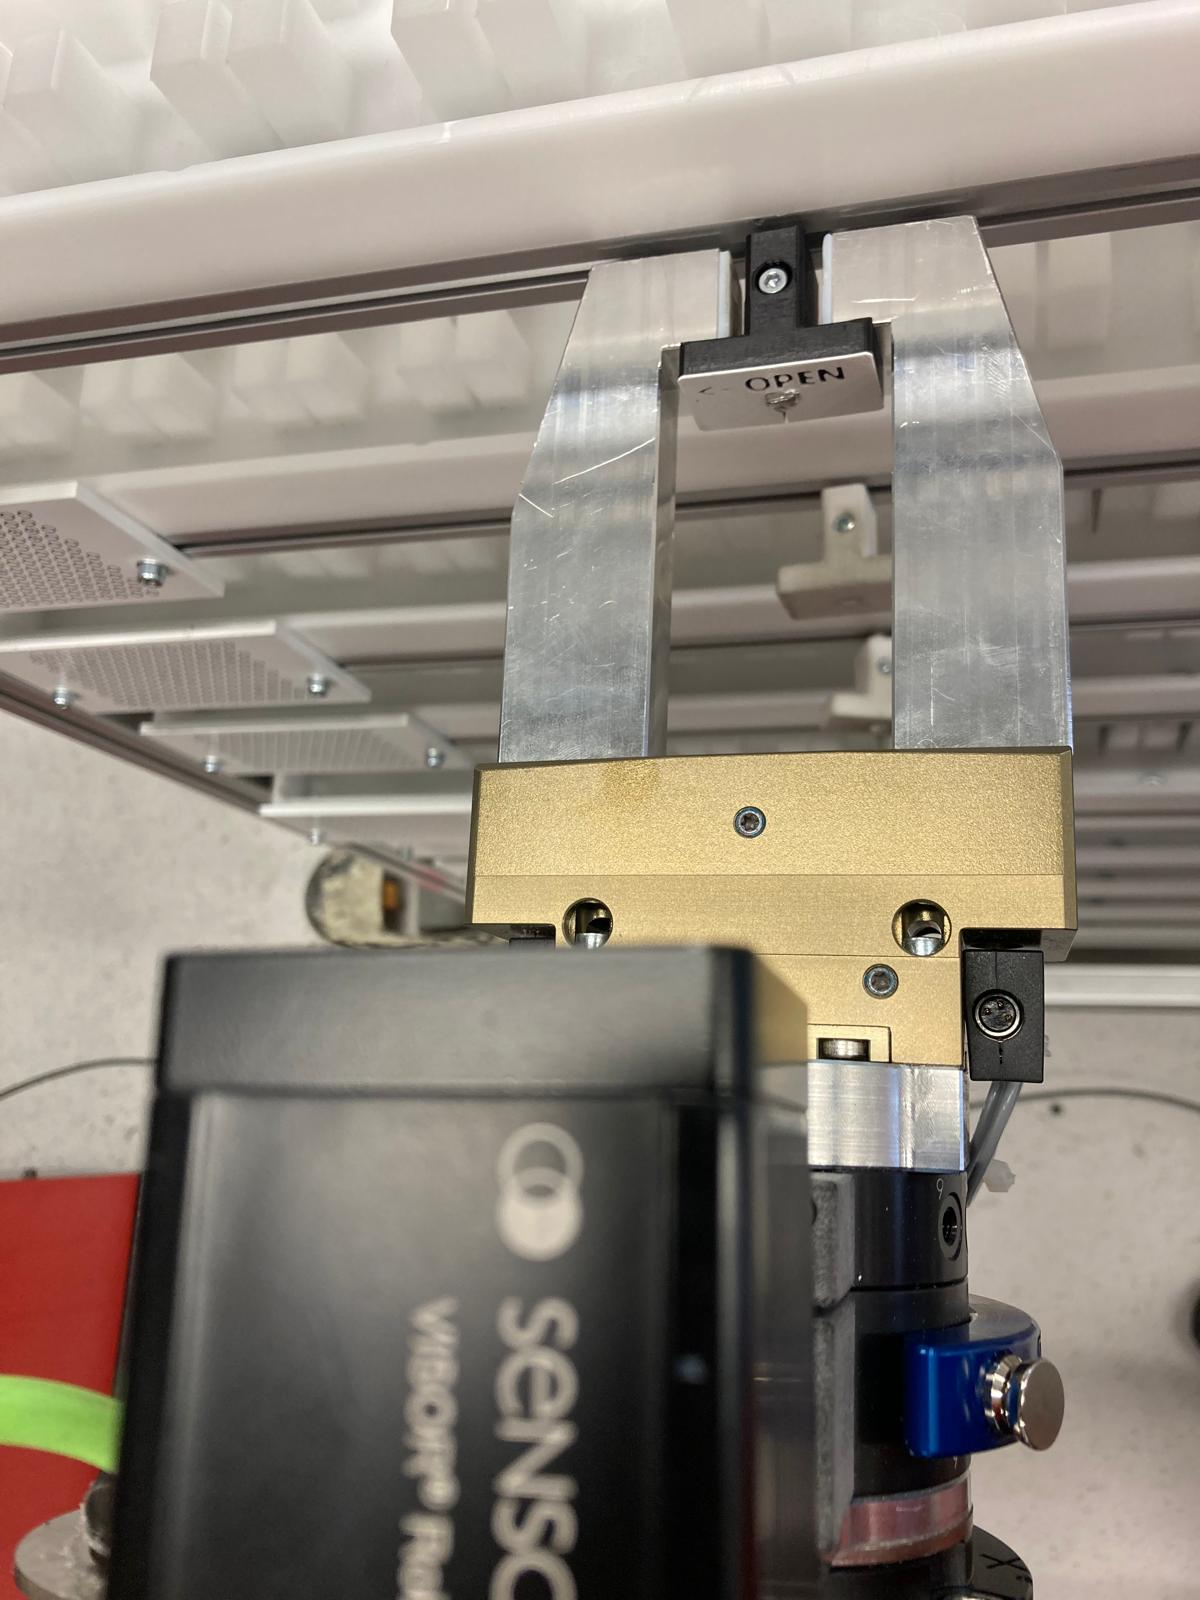
\includegraphics[width=\textwidth]{figures/shelf-control/hold-handle.jpeg}
        \caption{grasp handle with gripper}
        \label{subfig:grasp-handle}
    \end{subfigure}\hspace{0.1cm}
    \vspace{1cm}
    \begin{subfigure}[b]{0.32\textwidth}
        \centering
        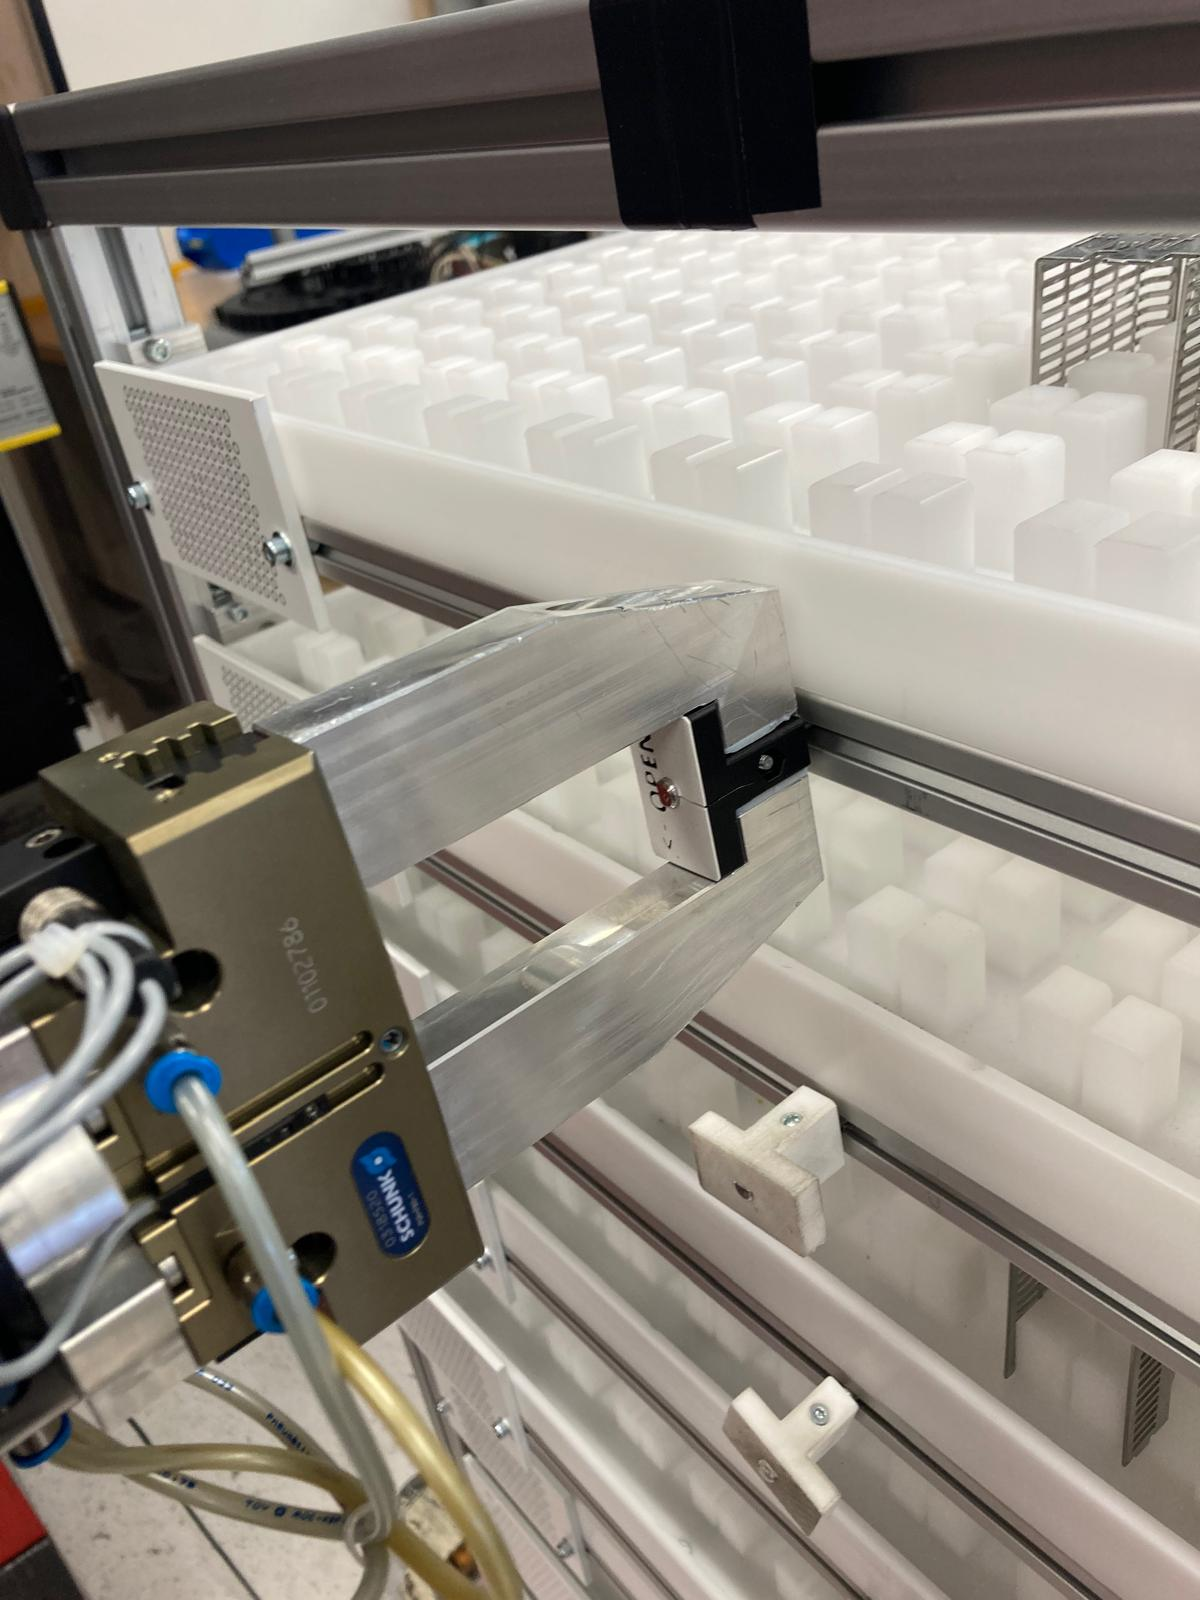
\includegraphics[width=\textwidth]{figures/shelf-control/open-handle.jpeg}
        \caption{Turn handle 100\textdegree{} to open drawer}
        \vspace{-0.45cm}
        \label{subfig:turn-open}
    \end{subfigure}\hspace{0.1cm}
    \begin{subfigure}[b]{0.32\textwidth}
        \centering
        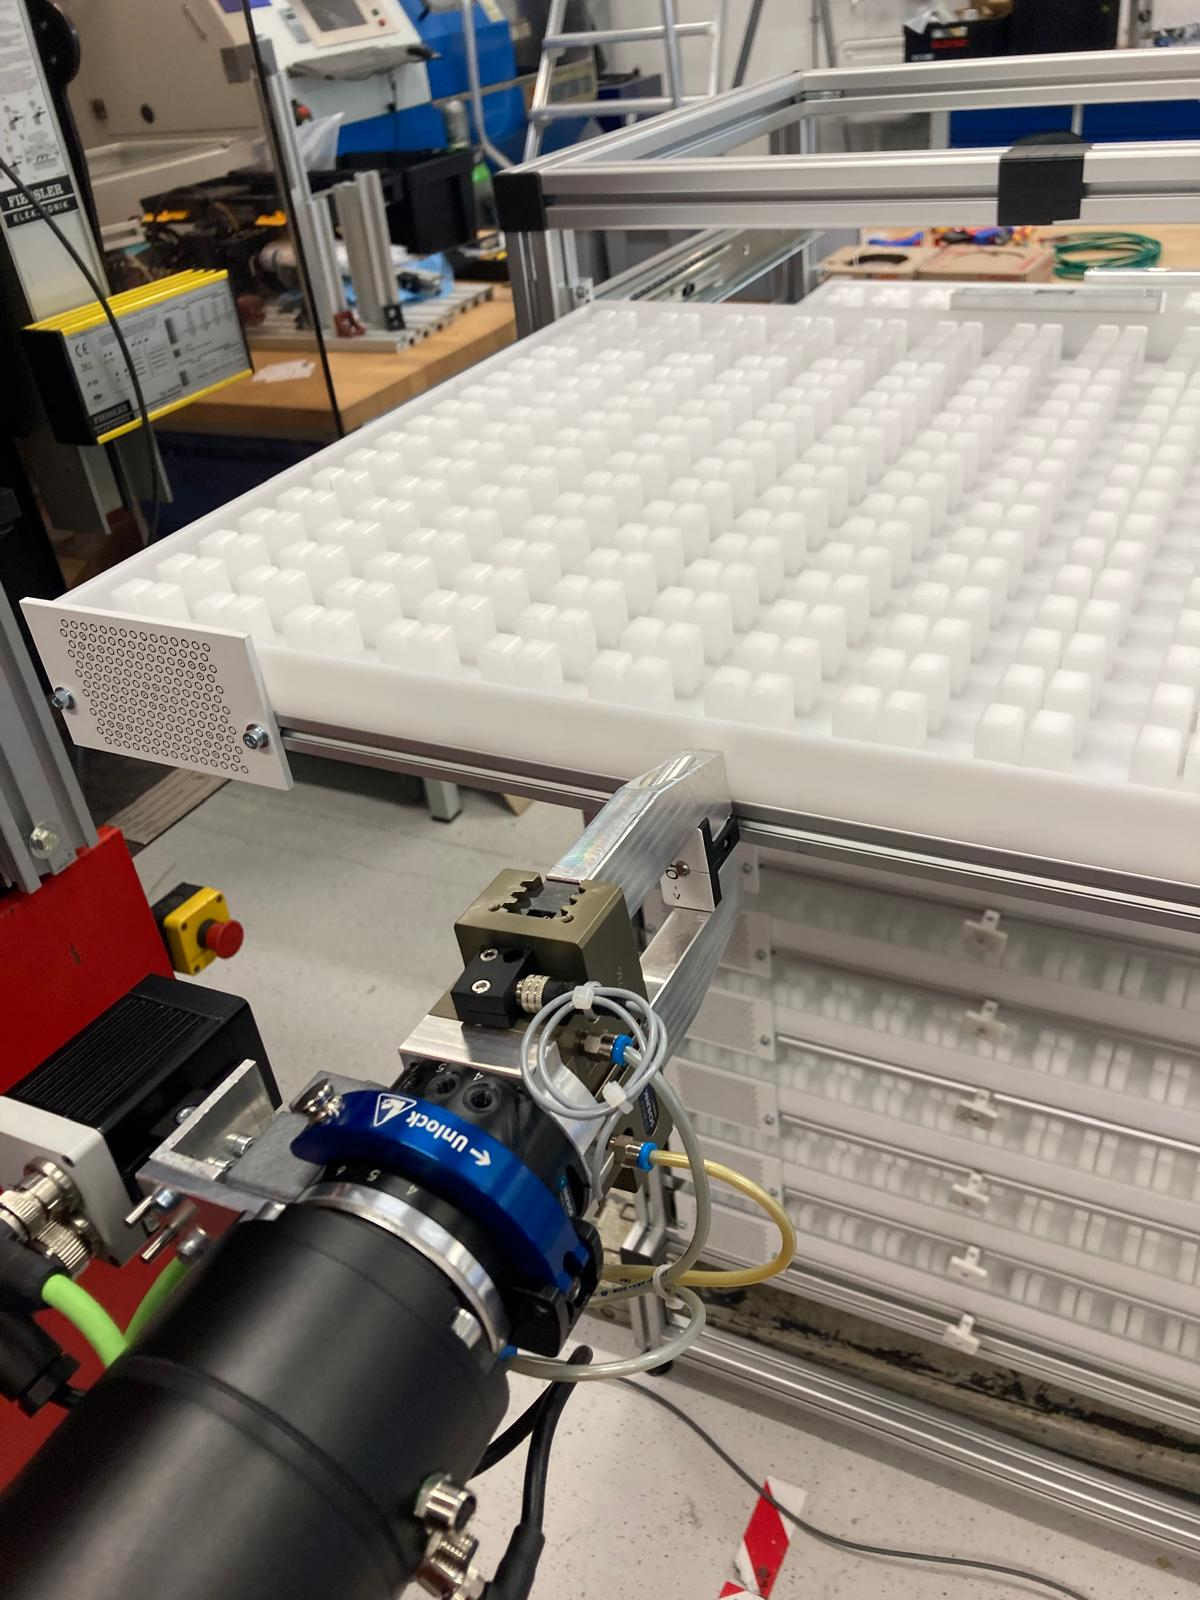
\includegraphics[width=\textwidth]{figures/shelf-control/open-drawer.jpeg}
        \caption{open drawer}
        \vspace{0.45cm}
        \label{fig:open-drawer}
    \end{subfigure}\hspace{0.1cm}
    \vspace{0.75cm}
    \begin{subfigure}[b]{0.32\textwidth}
        \centering
        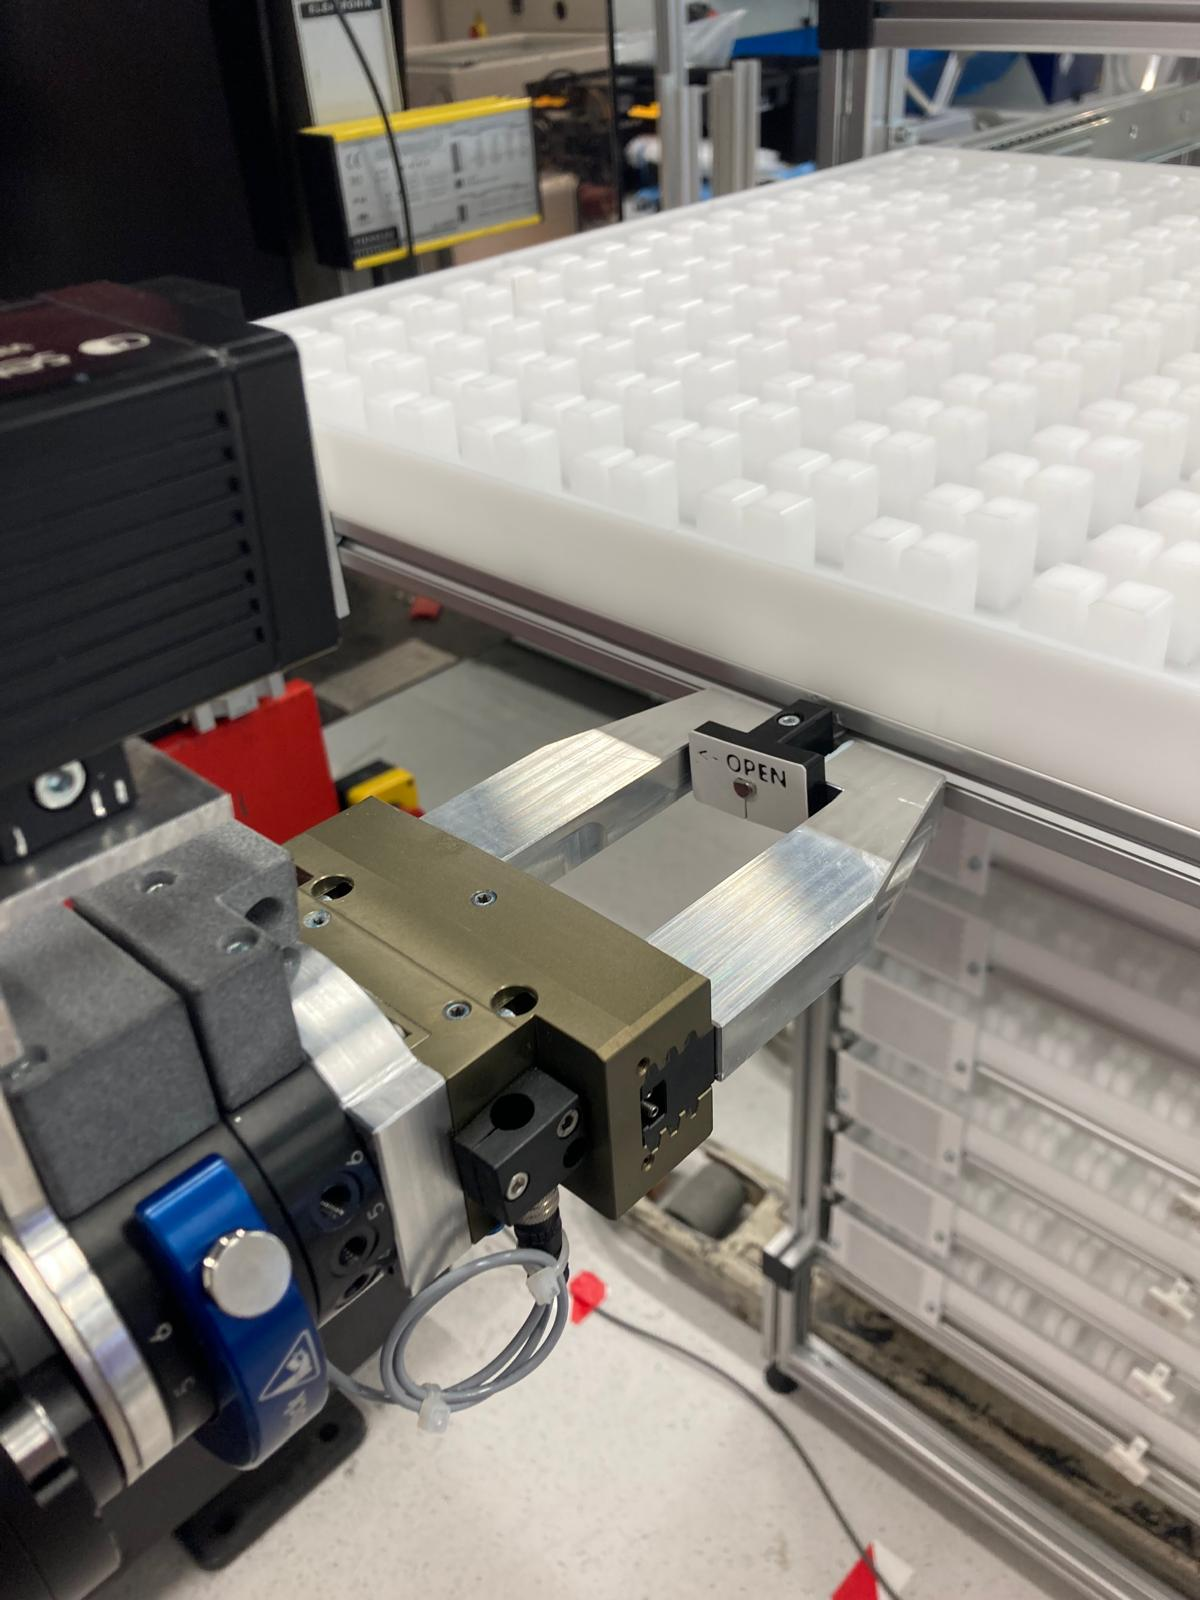
\includegraphics[width=\textwidth]{figures/shelf-control/close-handle.jpeg}
        \caption{Turn handle -100\textdegree{} to fix drawer in closed position}
        \label{fig:close-handle}
    \end{subfigure}\hspace{0.1cm}
    \begin{subfigure}[b]{0.32\textwidth}
        \centering
        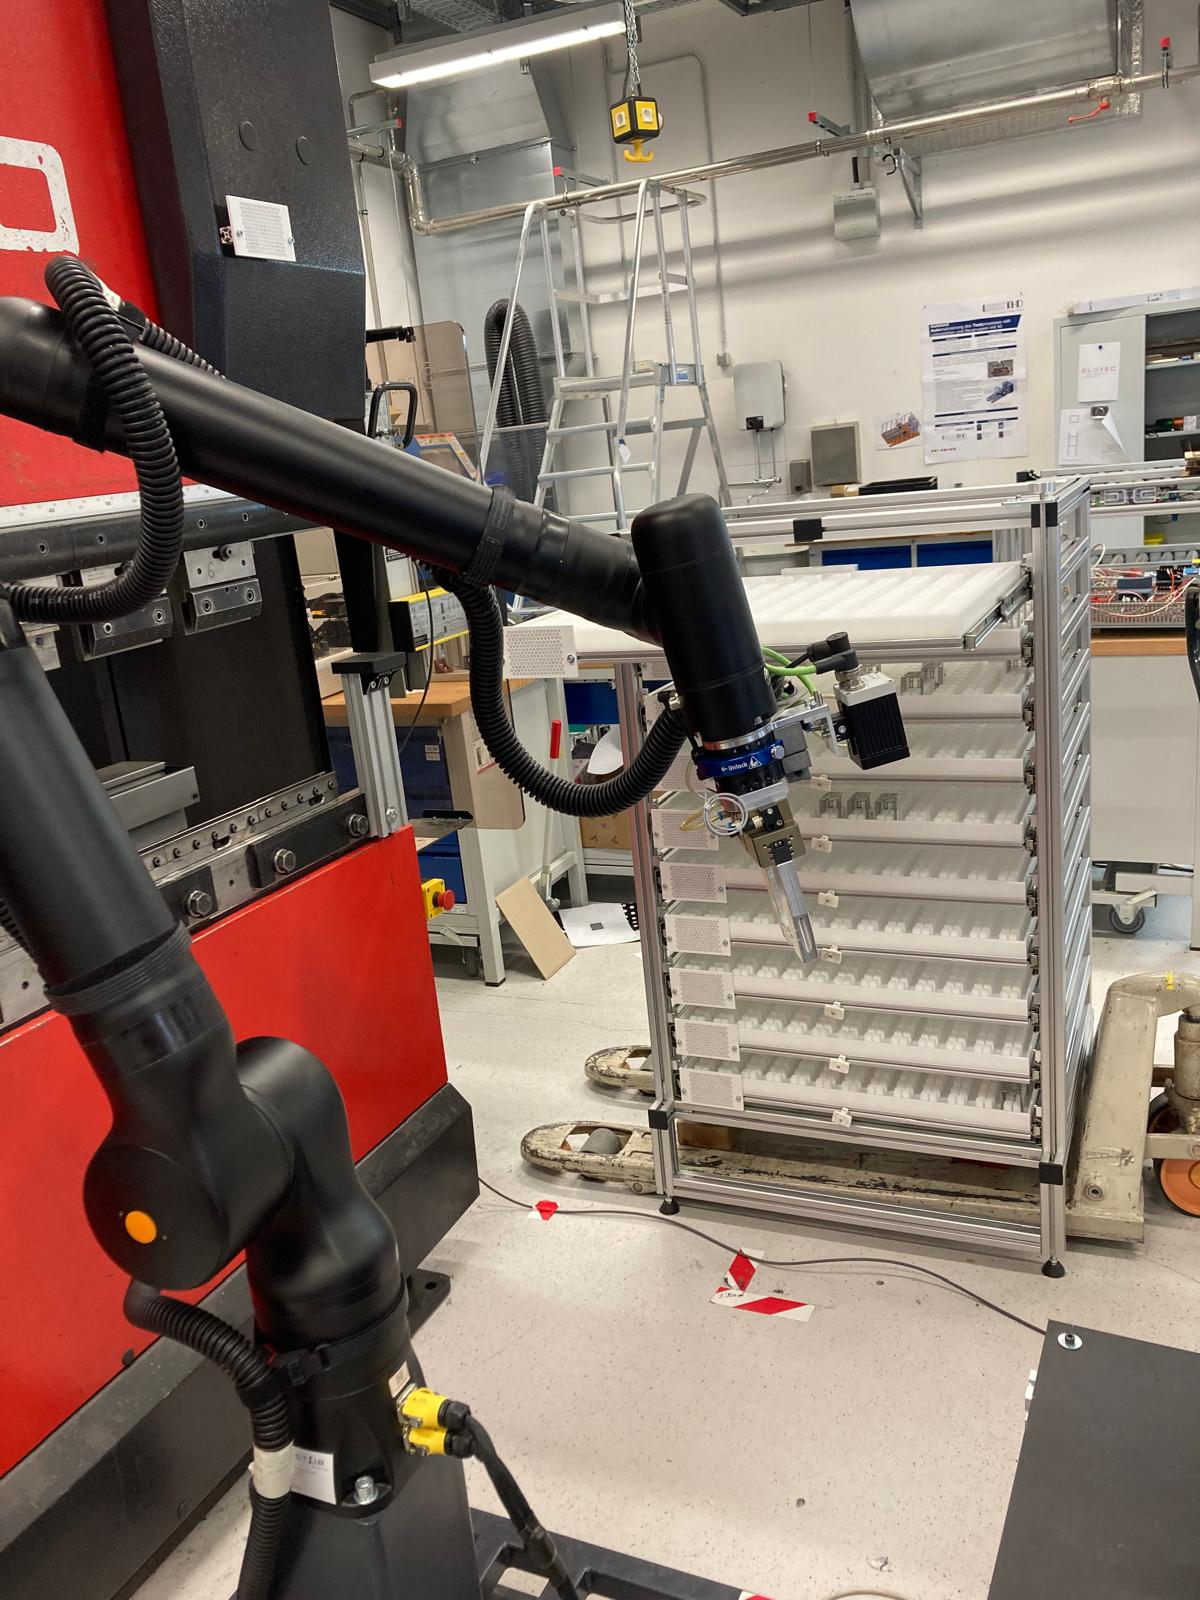
\includegraphics[width=\textwidth]{figures/shelf-control/drawer-opened.jpeg}
        \caption{Robot ready with drawer open}
        \label{subfig:drawer-opened}
    \end{subfigure}\hspace{0.1cm}
    \caption{Opening a shelf drawer for placement of bent sheet metal parts}
    \label{fig:shelf-control}
\end{figure}



\begin{figure}[h]
    \centering
    \begin{subfigure}[b]{0.48\textwidth}
        \centering
        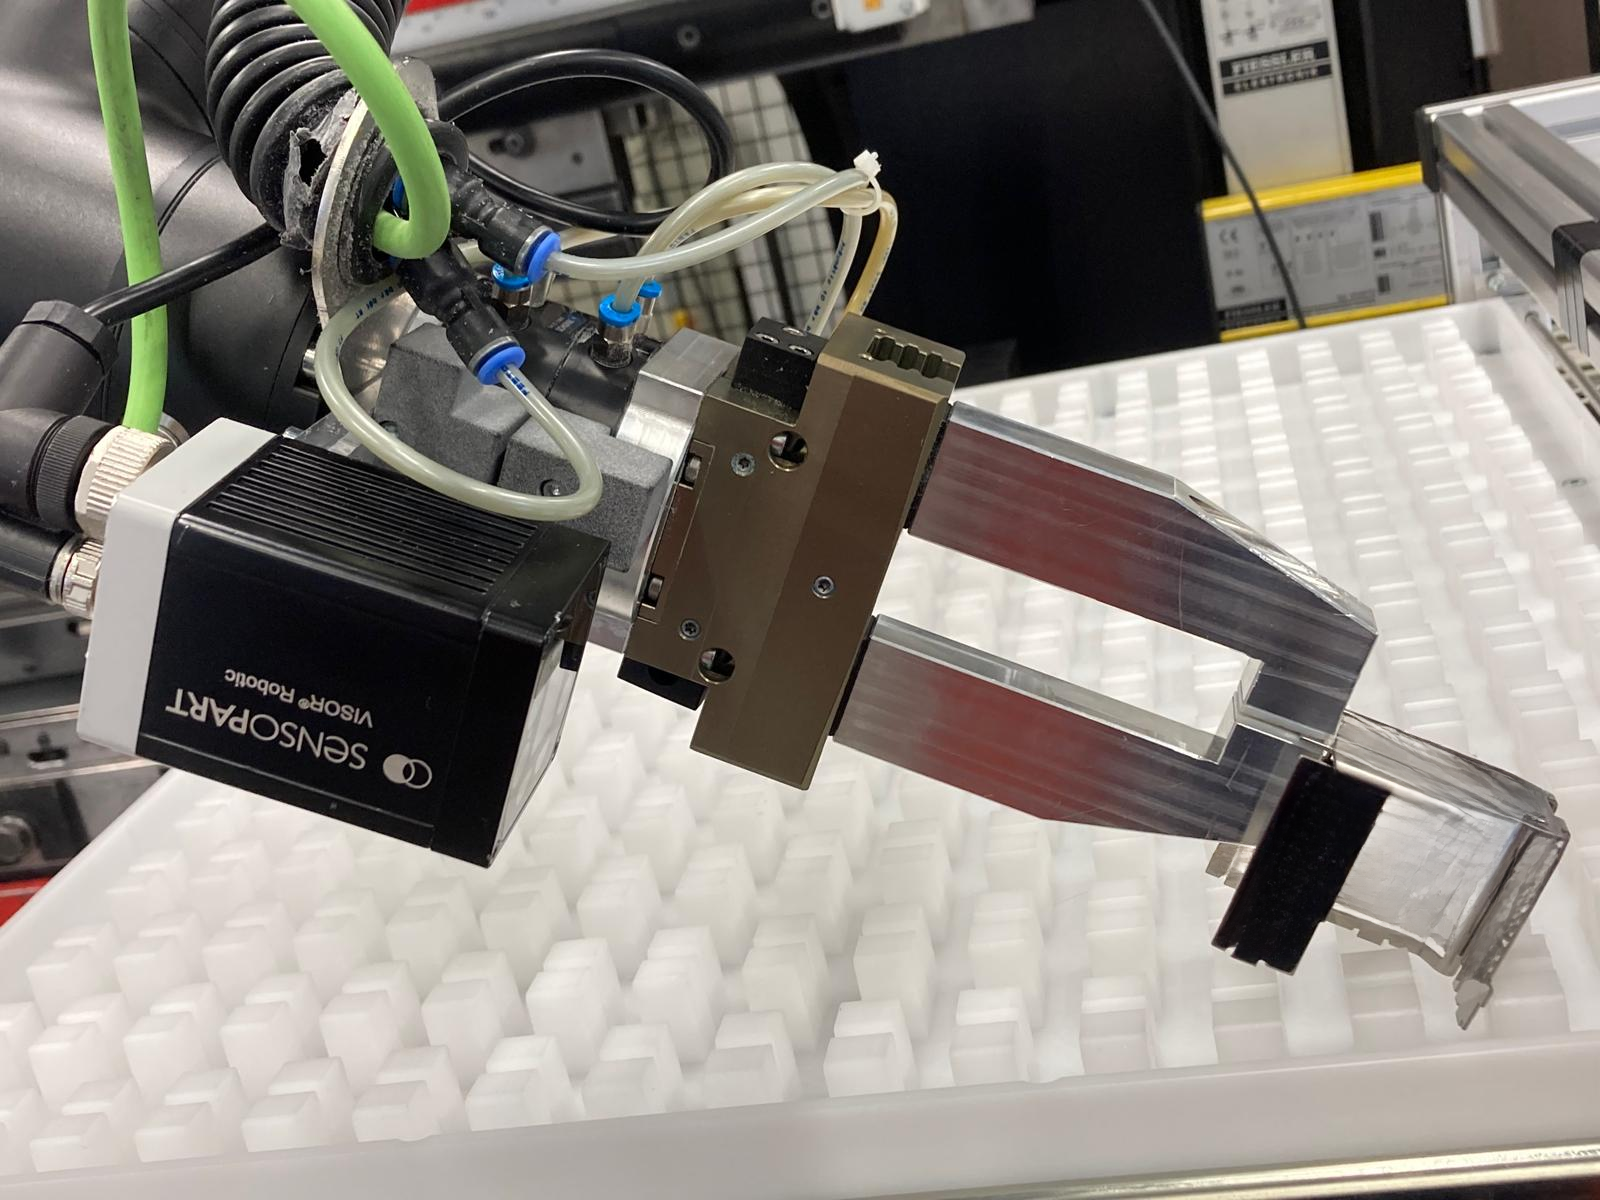
\includegraphics[width=\textwidth]{figures/shelf-control/sheet-placement-01.png}
        \caption{place bent sheet}
        \label{subfig:sheet-placement1}
    \end{subfigure}\hspace{0.1cm}
    \begin{subfigure}[b]{0.48\textwidth}
        \centering
        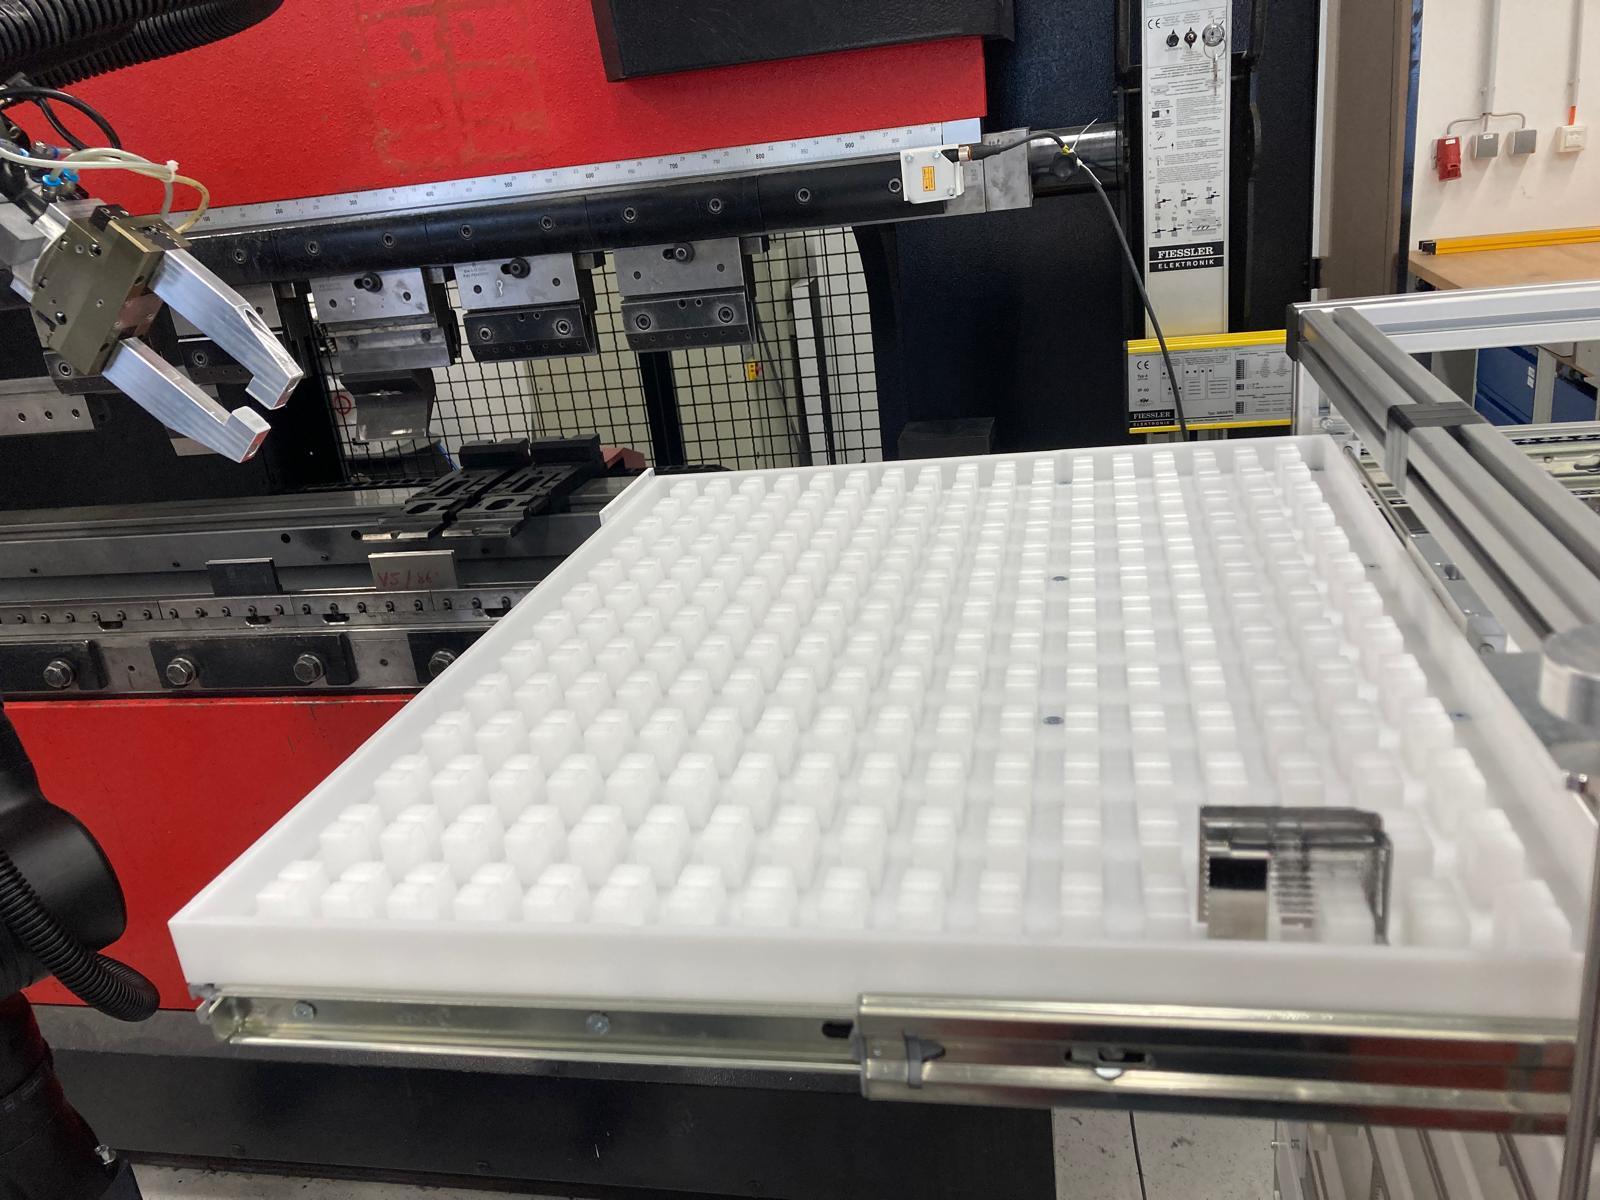
\includegraphics[width=\textwidth]{figures/shelf-control/sheet-placement-02.png}
        \caption{final position}
        \label{subfig:sheet-placement2}
    \end{subfigure}\hspace{0.1cm}
    \caption{Sheet placement}
    \label{fig:sheet-placement}
\end{figure}


